\documentclass[12pt, letterpaper]{article}
\usepackage[utf8]{inputenc}

\usepackage{hyperref}
\usepackage{changepage}   % for the adjustwidth environment

\usepackage{graphicx}
\usepackage{subfig}
\usepackage{float}

\usepackage{mathptmx}
\usepackage{indentfirst}
\usepackage{geometry}
 \geometry{
 left=2.5cm,
 right=2.5cm,
 top=2.5cm,
 bottom=2.5cm,
 }

\renewcommand*\descriptionlabel[1]{\hspace\leftmargin$#1$}

\title{Fluidos Template}
\author{Patricio López}
\date{May 2015}

\linespread{1}
\setlength\parindent{0.49cm}

\begin{document}

\section{Sección}

\subsection{Subsección}

Lorem ipsum dolor sit amet, consectetur adipisicing elit, sed do eiusmod
tempor incididunt ut labore et dolore magna aliqua. Ut enim ad minim veniam,
quis nostrud exercitation ullamco laboris nisi ut aliquip ex ea commodo
consequat.

\medskip

Duis aute irure dolor in reprehenderit in voluptate velit esse
cillum dolore eu fugiat nulla pariatur. Excepteur sint occaecat cupidatat non
proident, sunt in culpa qui officia deserunt mollit anim id est laborum. Footnote.\footnote{Compile LaTeX online on Sharelatex: \url{https://www.sharelatex.com}}


\subsection{Citas}

Cita por el autor P. Pérez:
\medskip
\begin{adjustwidth}{2cm}{}
    Lorem ipsum dolor sit amet, consectetur adipisicing elit, sed do eiusmod
    tempor incididunt ut labore et dolore magna aliqua. Ut enim ad minim veniam,
    quis nostrud exercitation ullamco laboris nisi ut aliquip ex ea commodo
    consequat. (Fecha, p. 4).
\end{adjustwidth}

\medskip

Lorem ipsum dolor ``consectetur adipisicing elit, sed do eiusmod tempor incididunt ut labore et dolore magna aliqua' (Fuente, 2015).

\subsection{Matemática}

Ecuación:
\begin{enumerate}
\item $\oint_C \! \stackrel{\rightarrow}{E} \stackrel{\rightarrow}{dl} = -\frac{d}{dt} \int_S \stackrel{\rightarrow}{B}\stackrel{\rightarrow}{dA} = \frac{-d\Phi}{dt}$
\item $V_\epsilon = -N\frac{d\Phi}{dt}$
\end{enumerate}

Símbolos:

\begin{itemize}
\item $E$: Electric field
\item $B$: Magnetic field
\item $V_\epsilon$: Electromotive force
\item $N$: Number of bobine spins
\item $\Phi$: Magnetic flow
\end{itemize}


\subsection{Imágenes}

Figura:

\begin{figure}[H]
    \centering
    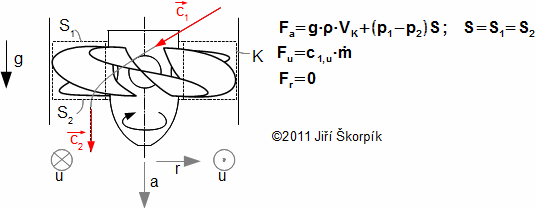
\includegraphics[width=10cm]{media/turbine_force.png}
    \caption{Caption}
\end{figure}



\newpage

\section*{Bibliografía}

\sloppy  % http://tex.stackexchange.com/questions/54946/how-to-break-long-url-in-an-item

\begin{enumerate}

\item Rouse, H. 2015. Books at Iowa: Highlights in the History of Hydraulics. Digital.lib.uiowa.edu [en línea]. [Consulta: 26 mayo 2015]. Disponible en: \url{http://digital.lib.uiowa.edu/bai/hydraul.htm}.

\end{enumerate}

\end{document}
